\documentclass[11pt,a4paper]{article}
\usepackage[margin=19mm,top=20mm,bottom=20mm]{geometry}
\usepackage{amsmath,amssymb,graphicx,array,fancyhdr,lastpage,textcomp,fancyvrb}
\usepackage{fontspec}
\usepackage[hidelinks]{hyperref}
\setmainfont{texgyreheros-regular.otf}[BoldFont=texgyreheros-bold.otf,ItalicFont=texgyreheros-italic.otf,BoldItalicFont=texgyreheros-bolditalic.otf]
\setmonofont{lmmono10-regular.otf}
\setlength{\parindent}{0pt}\setlength{\parskip}{5pt}
\setlength{\headheight}{14pt}
\pagestyle{fancy}\fancyhf{}
\renewcommand{\headrulewidth}{0.3pt}\renewcommand{\footrulewidth}{0.3pt}
\fancyfoot[L]{\footnotesize by paper.shrit.in\quad |\quad normal}
\fancyfoot[R]{\footnotesize Page \thepage\ of \pageref{LastPage}}
\begin{document}
\fancyhead[L]{\small Data Analytics}\fancyhead[R]{\small Set B: Original}
{\LARGE\bfseries Worked Solutions}\par{\large Data Analytics}\par\textbf{Set B: Original | CSE Semester 3}\par
Companion to \texttt{da-original.pdf}. Question numbers match that paper. Equivalent correct methods are acceptable. These are independent worked solutions, not an official university marking scheme.\par\medskip\hrule\medskip
Questions 1--5: MCQ answer key, 1 mark each (5 marks total). Questions 6 onward: theory solutions (25 marks total).\par
\noindent\begin{minipage}{\linewidth}\subsection*{1. Arithmetic mean}
\textbf{Correct option: (C).} The sum is 48 and $48/6=8$.
\end{minipage}\par\medskip
\noindent\begin{minipage}{\linewidth}\subsection*{2. Median}
\textbf{Correct option: (B).} The middle values are 6 and 8, so the median is $(6+8)/2=7$.
\end{minipage}\par\medskip
\noindent\begin{minipage}{\linewidth}\subsection*{3. Population variance}
\textbf{Correct option: (A).} Population variance divides the squared-deviation sum by $N$: $64/6$.
\end{minipage}\par\medskip
\noindent\begin{minipage}{\linewidth}\subsection*{4. Pearson skewness sign}
\textbf{Correct option: (D).} $3(\bar x-\mathrm{median})/\sigma=3(8-7)/\sigma>0$.
\end{minipage}\par\medskip
\noindent\begin{minipage}{\linewidth}\subsection*{5. Resistance to extremes}
\textbf{Correct option: (B).} The median depends on the middle ranks and is generally more resistant to extremes.
\end{minipage}\par\medskip
\noindent\begin{minipage}{\linewidth}\subsection*{6. Five-number summary and outlier}

The median is 9. Excluding it gives lower half $(3,5,7,8)$ and upper half $(11,13,16,30)$.
Thus $Q_1=6$, $Q_3=14.5$, and the five-number summary is $\boxed{(3,6,9,14.5,30)}$.
$IQR=8.5$; the fences are $-6.75$ and $27.25$. Therefore 30 is an outlier. The modified box plot has whiskers at 3 and 16, with 30 plotted separately.
\begin{center}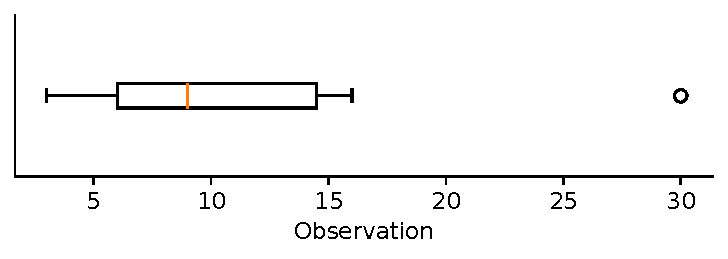
\includegraphics[width=.75\linewidth]{figures/box-original.pdf}\end{center}
\end{minipage}\par\medskip
\noindent\begin{minipage}{\linewidth}\subsection*{7. Missing and inconsistent data}

Impute missing ages with the median of a relevant, sufficiently large customer group and retain a missingness flag. Estimate imputation values from training data only if building a predictive model. Flag rows where annual income differs materially from $12\times$ monthly income after aligning currency, units, gross/net definitions and time period. Investigate such rows rather than automatically overwriting them.
\end{minipage}\par\medskip
\noindent\begin{minipage}{\linewidth}\subsection*{8. Filling-machine mean test}

$H_0:\mu=500$ ml, $H_1:\mu\ne500$ ml. The standard error is $12/\sqrt{36}=2$ ml.
\[z=\frac{496-500}{2}=\boxed{-2.00}.\]
Since $|-2|>1.96$, reject $H_0$ at 5\%. There is evidence that the machine's mean fill differs from 500 ml; the sample suggests underfilling. The two-sided $p$-value is about 0.0455.
\end{minipage}\par\medskip
\noindent\begin{minipage}{\linewidth}\subsection*{9. Rank correlation}

The six rank differences are $(-1,1,-1,1,-1,1)$, giving $\sum d_i^2=6$.
\[r_s=1-\frac{6(6)}{6(6^2-1)}=\boxed{\frac{29}{35}=0.8286}.\]
There is strong positive rank agreement, although each adjacent pair is reversed.
\end{minipage}\par\medskip
\noindent\begin{minipage}{\linewidth}\subsection*{10. Equal-frequency smoothing}
\begin{center}\renewcommand{\arraystretch}{1.2}\begin{tabular}{lll}\hline Bin & Observations & Mean\\\hline
1 & 10,12,15,18 & 55/4 = 13.75\\
2 & 20,22,25,28 & 95/4 = 23.75\\
3 & 30,32,35,40 & 137/4 = 34.25\\\hline\end{tabular}\end{center}The smoothed sequence is four copies of 13.75, followed by four copies of 23.75 and four copies of 34.25.
\end{minipage}\par\medskip
\noindent\begin{minipage}{\linewidth}\subsection*{11. Training and passing}

$H_0$: training and passing are independent. Row totals are 60 and 40; column totals are 70 and 30. Expected counts are
\[E=\begin{pmatrix}42&18\\28&12\end{pmatrix}.\]
\[\chi^2=\frac{(48-42)^2}{42}+\frac{(12-18)^2}{18}
+\frac{(22-28)^2}{28}+\frac{(18-12)^2}{12}
=\boxed{7.1429}.\]
With one degree of freedom, $7.1429>3.841$, so reject independence. Training and passing are associated. The pass rates are 80\% and 55\%; causation requires an appropriate study design.
\end{minipage}\par\medskip
\noindent\begin{minipage}{\linewidth}\subsection*{12. One-way ANOVA}
\begin{center}\renewcommand{\arraystretch}{1.2}\begin{tabular}{lllll}\hline Source & SS & df & MS & F\\\hline
Between & 54 & 2 & 27 & 27\\
Within & 6 & 6 & 1 & \\
Total & 60 & 8 &  & \\\hline\end{tabular}\end{center}Test $H_0:\mu_A=\mu_B=\mu_C$. Since $F=27>5.143$, reject $H_0$ at 5\%. At least one population mean differs. Pairwise differences require further testing.
\end{minipage}\par\medskip
\noindent\begin{minipage}{\linewidth}\subsection*{13. Type I and Type II errors}

A Type I error is rejecting $\mu=500$ when the machine's true mean is 500 ml. A Type II error is failing to reject $\mu=500$ when the true mean differs from 500 ml. The 5\% significance level controls the Type I error probability under the test assumptions; it does not specify the Type II probability.
\end{minipage}\par\medskip

\end{document}
